\documentclass[a4paper]{jpconf}

\usepackage{graphicx}
\usepackage{bm}        % for math
\usepackage{amssymb}   % for math
\usepackage{amsfonts}
\usepackage{amsmath}
\usepackage{epsfig}
\usepackage{units}
\usepackage{cite}
%\usepackage[numbers,square,sort&compress]{natbib}
\usepackage[utf8]{inputenc}
\usepackage[T1]{fontenc}
\usepackage{color}
\usepackage{hyperref}

%particles
\newcommand{\jpsi}{\rm J/$\psi$}
\newcommand{\psip}{$\psi^\prime$}
\newcommand{\jpsiDY}{\rm J/$\psi$\,/\,DY}
\newcommand{\chic}{$\chi_{\rm c}$}
\newcommand{\pip}{$\pi^{+}$}
\newcommand{\pim}{$\pi^{-}$}
\newcommand{\pizero}{$\pi^{0}$}
\newcommand{\kap}{K$^{+}$}
\newcommand{\kam}{K$^{-}$}
\newcommand{\pbar}{$\rm\overline{p}$}
\newcommand{\ccbar}{\ensuremath{\mathrm{c\overline{c}}}}
\newcommand{\bbbar}{\ensuremath{\mathrm{b\overline{b}}}}
\newcommand{\Dzero}{\ensuremath{\mathrm{D^{0}}}}
\newcommand{\Dzerobar}{\ensuremath{\mathrm{\overline{D}^{0}}}}
\newcommand{\Dpm}{\ensuremath{\mathrm{D^{\pm}}}}
\newcommand{\Ds}{\ensuremath{\mathrm{D_{s}^{\pm}}}}
\newcommand{\Dstar}{\ensuremath{\mathrm{D^{*\pm}}}}

%collision systems
\newcommand{\pp}{pp}
\newcommand{\pPb}{p--Pb}
\newcommand{\PbPb}{Pb--Pb}

%detectors
\newcommand{\ezdc}{$E_{\rm ZDC}$}

%units
\newcommand{\GeVc}{GeV/$c$}
\newcommand{\GeVcsq}{GeV/$c^2$}

%others
\newcommand{\degree}{$^{\rm o}$}
\newcommand{\s}{\ensuremath{\sqrt{s}}}
\newcommand{\snn}{\ensuremath{\sqrt{s_{\rm NN}}}}
\newcommand{\y}{\ensuremath{y}}
\newcommand{\pt}{\ensuremath{p_{\rm T}}}
\newcommand{\dedx}{d$E$/d$x$}
\newcommand{\dndy}{d$N$/d$y$}
\newcommand{\dndydpt}{${\rm d}^2N/({\rm d}y {\rm d}p_{\rm t})$}
\newcommand{\zpar}{\ensuremath{z_{||}}}
\newcommand{\zpargen}{\ensuremath{z_{||}^{\mathrm{part}}}}
\newcommand{\zpardet}{\ensuremath{z_{||}^{\mathrm{det}}}}
\newcommand{\ptchjet}{\ensuremath{p_{\mathrm{T,ch\, jet}}}}
\newcommand{\ptjet}{\ensuremath{p_{\mathrm{T,jet}}}}
\newcommand{\ptchjetgen}{\ensuremath{p_{\mathrm{T,ch\,jet}}^{\mathrm{part}}}}
\newcommand{\ptchjetdet}{\ensuremath{p_{\mathrm{T,ch\,jet}}^{\mathrm{det}}}}
\newcommand{\ptd}{\ensuremath{p_{\mathrm{T,D}}}}
\newcommand{\ptdgen}{\ensuremath{p_{\mathrm{T,D}}^{\mathrm{part}}}}
\newcommand{\ptddet}{\ensuremath{p_{\mathrm{T,D}}^{\mathrm{det}}}}
\newcommand{\antikt}{anti-\ensuremath{k_{\mathrm{T}}}}
\newcommand{\Antikt}{Anti-\ensuremath{k_{\mathrm{T}}}}
\newcommand{\kt}{\ensuremath{k_{\mathrm{T}}}}
\newcommand{\pthard}{\ensuremath{p_{\mathrm{T,hard}}}}

\begin{document}
\title{Measurement of D-meson tagged jets in pp collisions at 7 TeV with ALICE}

\author{Salvatore Aiola, for the ALICE Collaboration}

\address{Physics Department, Yale University, 266 Whitney Avenue, New Haven, CT 06511}

\ead{salvatore.aiola@cern.ch}

\begin{abstract}
We present the current status of the measurement of jets that contain a D meson (D-tagged jets) with \mbox{ALICE}.
The aim of the analysis is to extract both the $p_{\rm T}$ spectrum of the D-tagged jets and the jet-momentum fraction of the D mesons. 
We identify D-meson candidates via their hadronic decay channels using topological selections and particle identification.
These D-meson candidates are combined with the other charged tracks reconstructed by the central tracking system, 
using the anti-$k_{\rm T}$ jet-finding algorithm.
We extract the yield of D-tagged jets through an invariant mass analysis of the D-meson candidates associated with each jet, 
in bins of jet $p_{\rm T}$.
A Monte Carlo simulation that uses PYTHIA6 as event generator and GEANT3 as transport code with a detailed description of the ALICE apparatus,
has been used to extract the detector performance and validate the signal extraction techniques.
\end{abstract}

\section{Introduction}
At hadron colliders, charm quarks are produced as a result of a hard scattering of partons. Like lighter quarks or gluons, charm quarks
fragment into collimated sprays of hadrons called \emph{jets}. The charm content of the jet is conserved throughout the fragmentation process,
which is dominated by Quantum Chromo-Dynamics (QCD).
%the theory of strong nuclear interactions;
In the final state, the charm content can be identified by looking for the presence of charmed hadrons.
%i.e. hadrons that have a charm quark among their valence quarks. Since all charmed hadrons have short lifetimes ($\tau \lesssim 10^{-12}$~s) their presence is inferred
%using a combination of Particle Identification (PID) techniques and selection of specific kinematics and topological patterns of their decay products.

The measurement of the charm jet production cross section in \pp\ collisions is an important, sensitive test of perturbative QCD (pQCD) calculations.
In particular, at the LHC energies, the measurement of charm production at low \pT\ probes the parton distribution functions (PDFs)
of the proton at small values of parton fractional momentum, $x$, and squared momentum transfer, $Q^2$, 
a kinematical region where pQCD calculations suffer from large uncertainties.
%For illustration, using a simplified $2 \rightarrow 2$ kinematics at leading order, c quarks ($m_{\mathrm{c}} \approx 1.5$~\GeVcsq) with
%$\pT \sim 2$~\GeVc\ and rapidity $y \sim 0$ probe the parton distribution functions at $x \sim 7 \times 10^{-4}$ and
%$Q^2 \sim (5~\mathrm{GeV})^2$.
%Perturbative QCD calculations have substantial uncertainties at low \pT, owing to both the large effect of the
%choice of the factorization and renormalization scales at low $Q^2$ and to the sizeable uncertainties on the
%gluon PDFs at small $x$~\cite{Cacciari:2015}. 
%The measurement of the charm differential cross section down to low \pT\ is relevant also for cosmic-ray and neutrino
%astrophysics: high-energy neutrinos from the decay of charmed hadrons produced in particle showers in the atmosphere constitute an important
%background for neutrinos from astrophysical sources~\cite{Gauld:2015, Bhattacharya:2015}.

Heavy quarks are also an ideal probe of the hot and dense matter, 
known as the Quark-Gluon Plasma (QGP)~\cite{STAR:2005a, PHENIX:2005a, ALICE:2010b, ALICE:2011b, CMS:2013d, ATLAS:2013c}, 
that is created in ultra-relativistic heavy-ion collisions. 
Hard scattered partons, including heavy quarks, are produced early in the collision. They interact with the QGP, which increases their virtuality and interferes with the
parton shower (\emph{jet quenching})~\cite{PHENIX:2003a, PHENIX:2008b, STAR:2003b, STAR:2003c, STAR:2006a, ALICE:2010d, CMS:2011c, CMS:2012b, ATLAS:2014d, ALICE:2015a}.
%can lead to a suppression of the jet yield, the disappearance of the back-to-back jet correlation peak,
%and a broadening and softening of the jet fragmentation. 
%A number of experimental results consistent with jet quenching have been reported in last decade
High-energy charm jets behave very much like jets that originate from light quarks; however at lower energies, comparable to the charm quark mass, the charm quark is expected
to interact less strongly with the QGP, a phenomenon known as the dead-cone effect~\cite{Dokshitzer:2001}.
%The measurement of the charm jet cross section in \pp\ collisions provides a baseline to look for collective effects in ultra-relativistic
%heavy-ion collisions. 
%In this context, another crucial aspect is the precise determination of the
%total charm-production cross section, needed to model charmonium regeneration in the QGP~\cite{Zhao:2011}.

Most of the charm-related measurements performed at the LHC so far report the production cross section of hadrons
containing heavy quarks~\cite{ALICE:2012d, ALICE:2012e, ATLAS:2012e, LHCb:2013a, ALICE:2014d, ATLAS:2014e, ALICE:2015c, ALICE:2015d, ALICE:2016a, ATLAS:2016a}.
Measuring the kinematic observables of jets implies integrating out some of the hadronization degrees of freedom. 
Since hadronization is a highly non-perturbative process, known only with large uncertainties~\cite{dEnterria:2014}, 
reducing its influence in the measurement may improve comparisons with pQCD calculations.
Furthermore, the details of the charm quark fragmentation can be the subject of a more careful study in which the kinematic observables 
of both the jet and the charmed hadron are available at the same time. In particular the measurement of the fraction of the jet momentum carried 
by the charmed hadron can provide important insights on the charm production mechanism~\cite{CDF:1990, UA1:1990, STAR:2009a, ATLAS:2012d}.

\section{The ALICE Experiment}
ALICE is the experiment dedicated to the study of heavy-ion collisions at the LHC.
The central barrel detectors are positioned within a large solenoid magnet, with a
field $B = 0.5$~T, parallel to the beam line and cover the mid-rapidity region ($\lvert \eta\rvert \lesssim 1$).
PID and low-momentum tracking capabilities are among the strongest points of ALICE~\cite{ALICE:2014b}.
The \emph{Inner Tracking System} (ITS) is a 6-layer silicon detector that allows the precise determination of the primary vertex and the displacement of 
secondary vertices of weak decays  enable measurement of the track impact parameter (i.e. the distance of
closest approach of the track to the primary interaction vertex) in the bending plane ($r\varphi$) with a resolution
better than $75, \rm \mu m$ for transverse momenta $\pT > 1$~\GeVc 

The main tracking detector is the \emph{Time Projection Chamber} (TPC), which, combined with the ITS, allows reconstruction of tracks down to $\pT=150$~\GeVc\ with a momentum resolution
of {\color{red} add resolution}. Several detectors contribute to the Particle Identification (PID) capabilities of ALICE. In particular for this measurement we use the \dedx\ measurement from the TPC and
the \emph{Time of Flight} (TOF) detector. The TOF is a {\color{red} add short description of TOF and time resolution}.
A full description of ALICE and of its performance during LHC Run-1 is available at Ref.~\cite{ALICE:2014b}.

\section{Analysis procedures}
The analysis relies on the well established D meson reconstruction techniques~\cite{ALICE:2012d, ALICE:2012e, ALICE:2014d, ALICE:2015c, ALICE:2015d, ALICE:2016a}, as well as
jet reconstruction methods~\cite{ALICE:2013c, ALICE:2014a, ALICE:2015e, ALICE:2015f}, both developed by the ALICE Collaboration. The analysis procedures are outlined in the following sections.

\subsection{Monte Carlo simulations}
ALICE plans to measure D-tagged jets in \pp\ collisions at $\s=$~7, 8 and 13 TeV and in \pPb\ and \PbPb\ collisions at $\snn=$~5 TeV.
Two Monte Carlo simulations have been used to extract the detector performance and validate the analysis techniques.

PYTHIA6 (6.4.28)~\ref{} (tune Perugia-{\color{red} check tune}) has been used as event generator in both simulations.
For the first simulation (minimum-bias production) PYTHIA was configured to provide Minimum Bias (MB) \pp\ events at $\s=7$~TeV.
The simulated statistics (about 300 M events) is close to the total statistics accumulated by ALICE in MB \pp\ collisions
in 2010. In the second simulation (charm-enhanced production) PYTHIA was configured to retain only events with a \ccbar\ pair; the production
was split in 8 \pthard\ bins, imposing a cut on the \pT\ of the hard scatted parton. In addition, all D meson were forced
to decay hadronically. These settings allowed to gain enough precision in the determination of the detector response with reasonable
computational costs.
In both cases, the PYTHIA events were then passed through the GEANT3 transport code with a detailed description of the ALICE apparatus,
as it was operated during the 2010 data-taking campaign.

\subsection{Track selection}
For more details about the tracking algorithm used by ALICE see Ref.~\cite{ALICE:2014b}.

Track quality cuts are applied to ensure good momentum resolution. These cuts
depend on the requirements set by a specific physics analysis.
Two types of tracks are used for this analysis. \emph{Global} tracks have the best
momentum and spatial resolution. They include at least one space point in the SPD (first two
layers of the ITS, closer to the beam pipe) and at least a total of three in the whole ITS. They are required also to
match with a track in the TPC, which has to include at least 70 space points and no less than 80\% of the geometrically findable 
space points in the TPC. Decay products of the D mesons are found among this category of tracks.

Due to the non-uniform SPD response, the reconstruction efficiency of the above defined \emph{global} tracks shows a strong azimuthal dependence.
This non-uniform acceptance can interfere with the jet-finding algorithm. To avoid such effects a second type of tracks is added for jet finding.
For this type of tracks the requirement on the SPD is lifted, while keeping all the other requirements unchanged. To improve momentum resolution,
these tracks are constrained to the primary vertex, which is reconstructed using \emph{global} tracks. This track collection is called \emph{hybrid} because
it includes a combination of \emph{global} tracks and \emph{constrained} tracks.

\subsection{D meson candidate identification}
ALICE has successfully measured a number of charmed mesons~\cite{ALICE:2012d, ALICE:2012e}.
The \Dzero\ meson has the best signal/background ratio down to low momentum and
is also the most abundant. The \Dzero\ has a mass $m=1.865$~\GeVcsq\ and a mean lifetime $\tau=4.101 \times 10^{-13}$~s.
It is identified through its hadronic decay: \Dzero $\rightarrow$ \pip \kam. The branching ratio of this decay
is relatively small, BR(\Dzero $\rightarrow$ \pip \kam) = 3.88\%~\cite{PDG:2014}. Both the \Dzero\ and its
anti-particle $\overline{\Dzero}$~are considered.

The first step of the analysis is to select events that contain at least one \Dzero\ meson candidate.
\Dzero\ meson candidates are identified looking for opposite-sign track pairs (\emph{daughters}) among all reconstructed \emph{global} tracks.
In order to suppress the background from combinatorial matches, topological and PID cuts are applied.
The topological cuts select pairs that form a \emph{secondary vertex} displaced from the reconstructed
primary vertex. 
PID information on the \Dzero\ candidate daughters is used to reject pairs that do not satisfy the requirement of being a pion-kaon pair.

The pairs that pass the selections are then used in the next steps.
The four-momentum of the \Dzero\ candidate is calculated summing the four-momenta of the two daughters.
When available, PID is used to assign mass values to the \Dzero\ candidate daughters. When PID is not conclusive,
the pair is used twice with either mass combinations (\pip \kam or \pim \kap). Using the four-momentum of the \Dzero\ candidate
the \emph{invariant mass} is calculated according to the usual special relativity formula: $m^2 = E^2 - \bm{p}^2$.

\subsection{Jet reconstruction}
For each \Dzero\ candidate a set of particle four-momenta is prepared and fed as input for the jet-finding algorithm.
This set includes the four-momentum of the \Dzero\ candidate and all reconstructed \emph{hybrid} tracks,
excluding the two daughters of the \Dzero. The jet-finding algorithm returns a set of jet candidates, with the particle constituents
assigned to each jet. The jet containing the \Dzero\ candidate can thus be identified and associated with the \Dzero\ candidate for the next steps.

For this analysis I use the \antikt\ algorithm~\cite{Cacciari:2008c}, widely used at the LHC.

Initially I will focus on using only tracks of charged particles for jet reconstruction. Since they miss the momentum
fraction carried by neutral particles, the kinematics of charged jets is less tightly correlated with the kinematics
of the original parton and depends more strongly on the jet fragmentation; however charged jets have also a number advantages
and have been the subject of recent theoretical developments~\cite{Thaler:2013}.
In a second phase I plan to extend the analysis by including the calorimeter data in jet finding (as done in Refs.~\cite{ALICE:2013c, ALICE:2015a}).

\subsection{Invariant mass analysis}
\Dzero\ candidates and their associated jets are then sorted according to their kinematic variables in different bins:
\begin{enumerate}
\item for a single-differential D-tagged jet \pT\ spectrum, the candidates will be divided in bins according to their associated jet \pT;
\item for a double-differential spectrum in jet \pT\ and \zpar$=\frac{\bm{p}_{\rm jet}\cdot{\bm{p}}_{\rm D^0}}{\bm{p}_{\rm jet}^2}$ candidates will
be sorted in bins defined in these two variables.
\end{enumerate}
For each bin defined above, a separate invariant mass analysis is performed. 
In each bin a fit of the invariant mass spectrum is performed to extract the signal from the background. It is assumed that the background has
a smooth shape that can be fitted by an exponential function, whereas the signal is fitted by a Gaussian. These assumptions are tested
through a Monte Carlo simulation that uses PYTHIA6~\cite{Sjostrand:2006} as particle generator and GEANT3~\cite{GEANT3-url} to simulate particle interaction
with the detector material budget and the detector response itself.

\subsection{Final corrections and systematic uncertainties}
Due to finite detector resolution, the spectrum obtained as outlined above is distorted. In addition the reconstruction efficiency is quite low
and \pT-dependent, especially for the D meson ($\epsilon_{D^0} \sim 10-20\%$, see Ref.~\cite{ALICE:2012d}). This is due both to the tracking efficiency ($\sim 80\%$, see Ref.~\cite{ALICE:2014b}),
which affects the probability of reconstructing the decay products, and to the topological cuts. These effects will be corrected for using a combination of Monte Carlo simulation and data-driven methods, currently being refined.
The corrections applied to remove or reduce effects due to detector resolution and efficiency are referred to as \emph{unfolding} and make use of modern statistical analysis methods~\cite{Hocker:1995, Dagostini:1995}.
A full \emph{closure} test using Monte Carlo simulated events is underway, to validate the ability of the analysis procedures to recover the signal.

Systematic uncertainties will be thoroughly assessed. Systematic uncertainties can arise from a variety of sources.
Some of the major sources come from irreducible inaccuracies in the assessment of the detector performance, in particular tracking efficiency, 
momentum resolution, primary/secondary vertex resolution, PID.
Other sources are more specific to the analysis procedures and are related to the invariant mass fits and to the unfolding techniques.

\section{Results}

\subsection{Detector performance}
The detector performance has been assessed using the charm-enhanced production. The D-tagged jets are identified at detector-level (i.e. after the GEANT3 detector response simulation)
in an way equivalent to real data processing, except for the invariant mass analysis step. The real D mesons are selected among the candidates using the MC truth.
The D-tagged jets are also identified at generator-level (i.e. PYTHIA events). Even-by-event, detector-level D-tagged jets are matched with their corresponding counter-parts at generator-level.
This matched pairs are used to build response matrices that relates detector-level observables with their corresponding particle-level observables. These matrices can be used
to correct detector-response distortions of the final distributions on an ensemble basis (\emph{unfolding}).

The jet momentum resolution and Jet Energy Scale (JES) shift have been quantified using the variable: 
\begin{equation}
\left( \ptchjetdet - \ptchjetgen \right) / \ptchjetgen, 
\end{equation}
where \ptchjetdet\ and \ptchjetgen are the transverse momenta of the D-tagged jet at detector-level and at generator-level, respectively.
Its probability density distribution is shown in Fig.~\ref{} for three different bins of \ptchjetgen. No significant dependence on \ptchjetgen\ is observed.
The shape of the distribution features a sharp peak at zero and is skewed towards negative values, due to tracking inefficiency (higher probability of
reconstructing jet momenta smaller than the generated ones). The relative jet momentum resolution is quantified with the standard deviation
of the probability density distribution in Fig.~\ref{}: $\sigma\approx$~\%. The relative JES shift can be quantified with the mean and the median of the same distribution:
mean~$\approx$~\% and median~$\approx$~\%. This values are comaprable to the ones obtained for inclusive jet~\cite{} for the same data-taking period, with a slightly better jet momentum resolution.

The reconstruction efficiency is calculated as the ratio of the yield of reconstructed D-tagged jets over all generated D-tagged jets, as a function of generator-level observables.
The reconstruction efficiency is shown in Fig.~\ref{} as a function of \ptd\ for different bins of \ptchjet. The reconstruction efficiency shows a stark dependence on \ptd\ mainly due to
tighter topological cuts applied at low momentum to suppress the D-meson combinatorial background. No significant dependence on \ptchjet\ is observed in the range $5<\ptchjet<24$~\GeVc.

\begin{figure}[h]
\centering
\begin{minipage}{.48\textwidth}
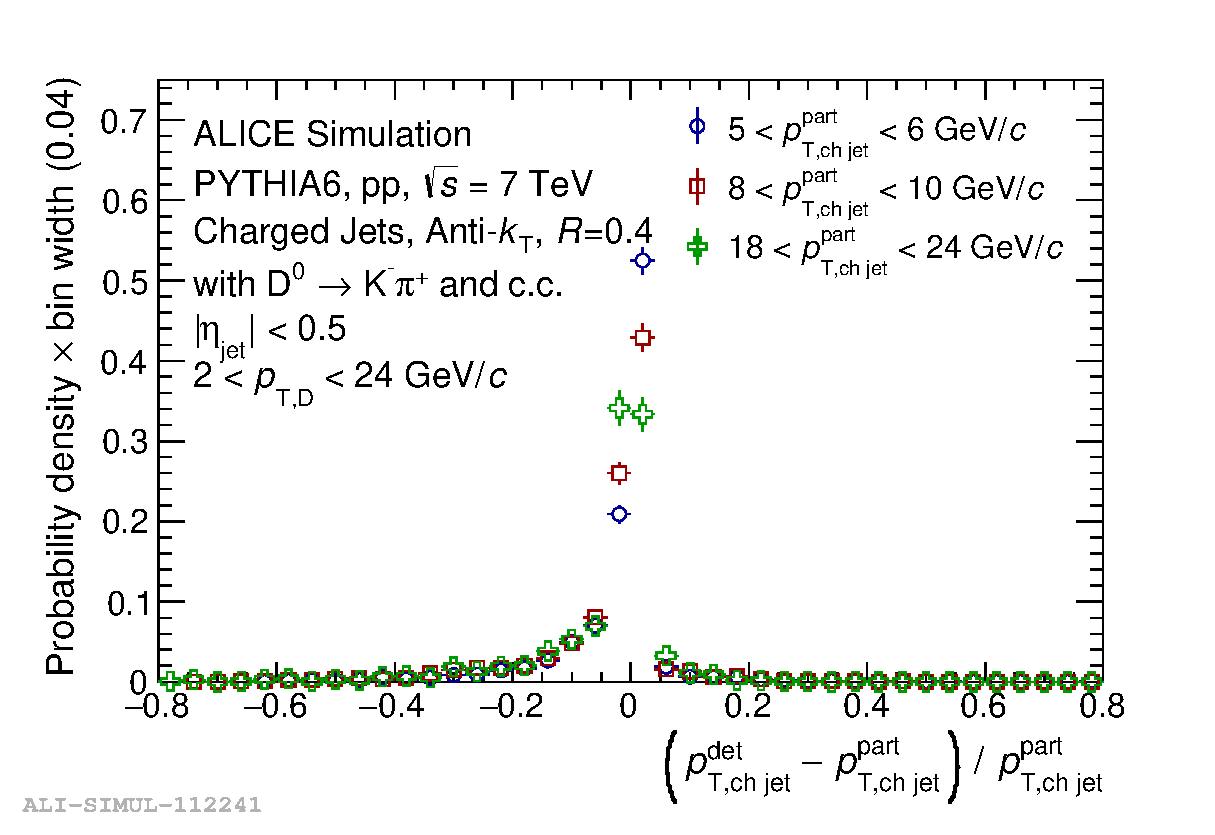
\includegraphics[width=\textwidth]{img/HQ16_Simulation_DetectorResponse}
\caption{\label{label}Figure caption for first of two sided figures.}
\end{minipage}\hspace{1pc}%
\begin{minipage}{.48\textwidth}
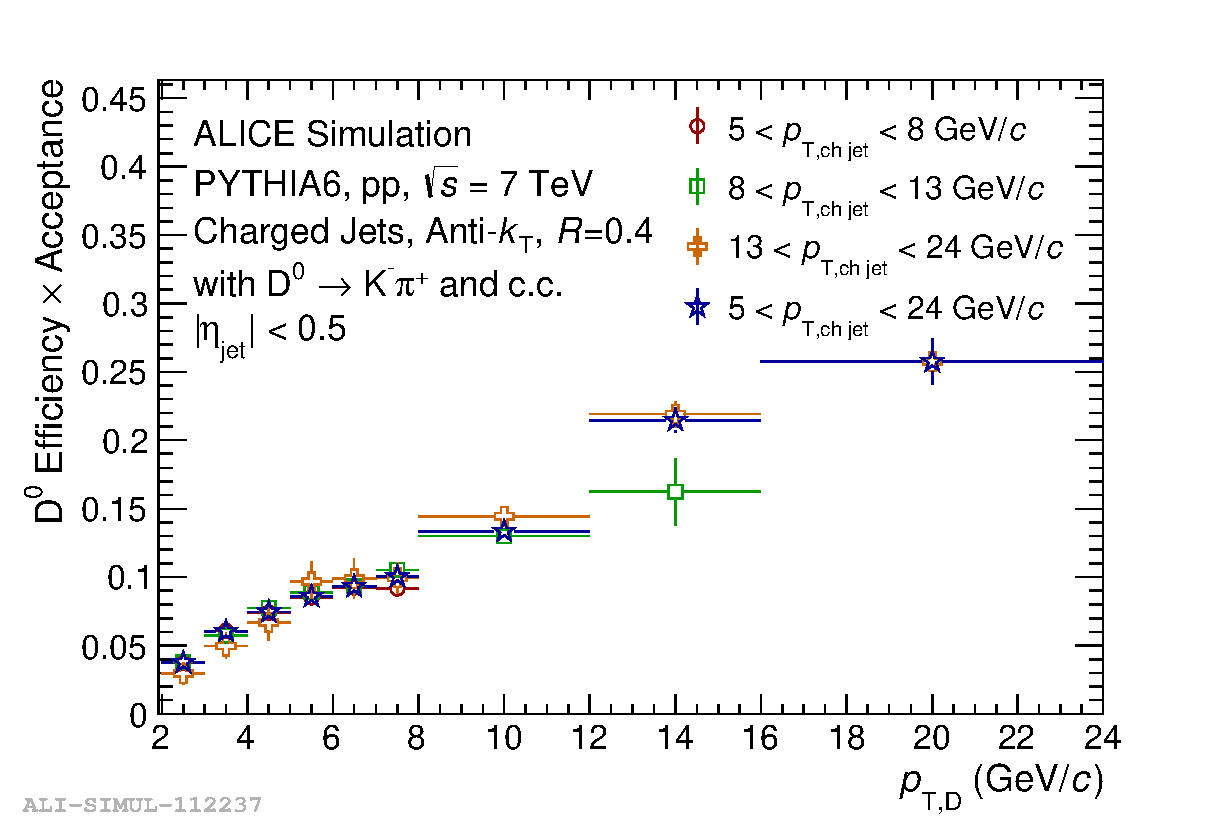
\includegraphics[width=\textwidth]{img/HQ16_Simulation_EfficiencyVsDPt}
\caption{\label{label}Figure caption for second of two sided figures.}
\end{minipage} 
\end{figure}

\subsection{Invariant mass analysis}
The minimum-bias production has been used to validate the invariant mass analysis. 
%Since this production has a similar statistics as the real data accumulated by ALICE in 2010 \pp\ data-taking, it provides a good guide to assess possible biases in the signal yield extraction. 
The D-tagged jets are identified at detector-level in an way equivalent to real data processing, including for the invariant mass analysis step.

Figure~\ref{} shows the D-tagged jet yields as a function of \ptchjetdet\ obtained using the invariant mass fit, side-band and like-sign background subtraction methods, compared to the yield obtained by selecting real D-tagged jets out of the 
combinatorial background using the MC truth. All methods seem to perform well and do not show any significant bias, beyond the statistical uncertainties connected to each of the signal extraction methods.

\begin{figure}[h]
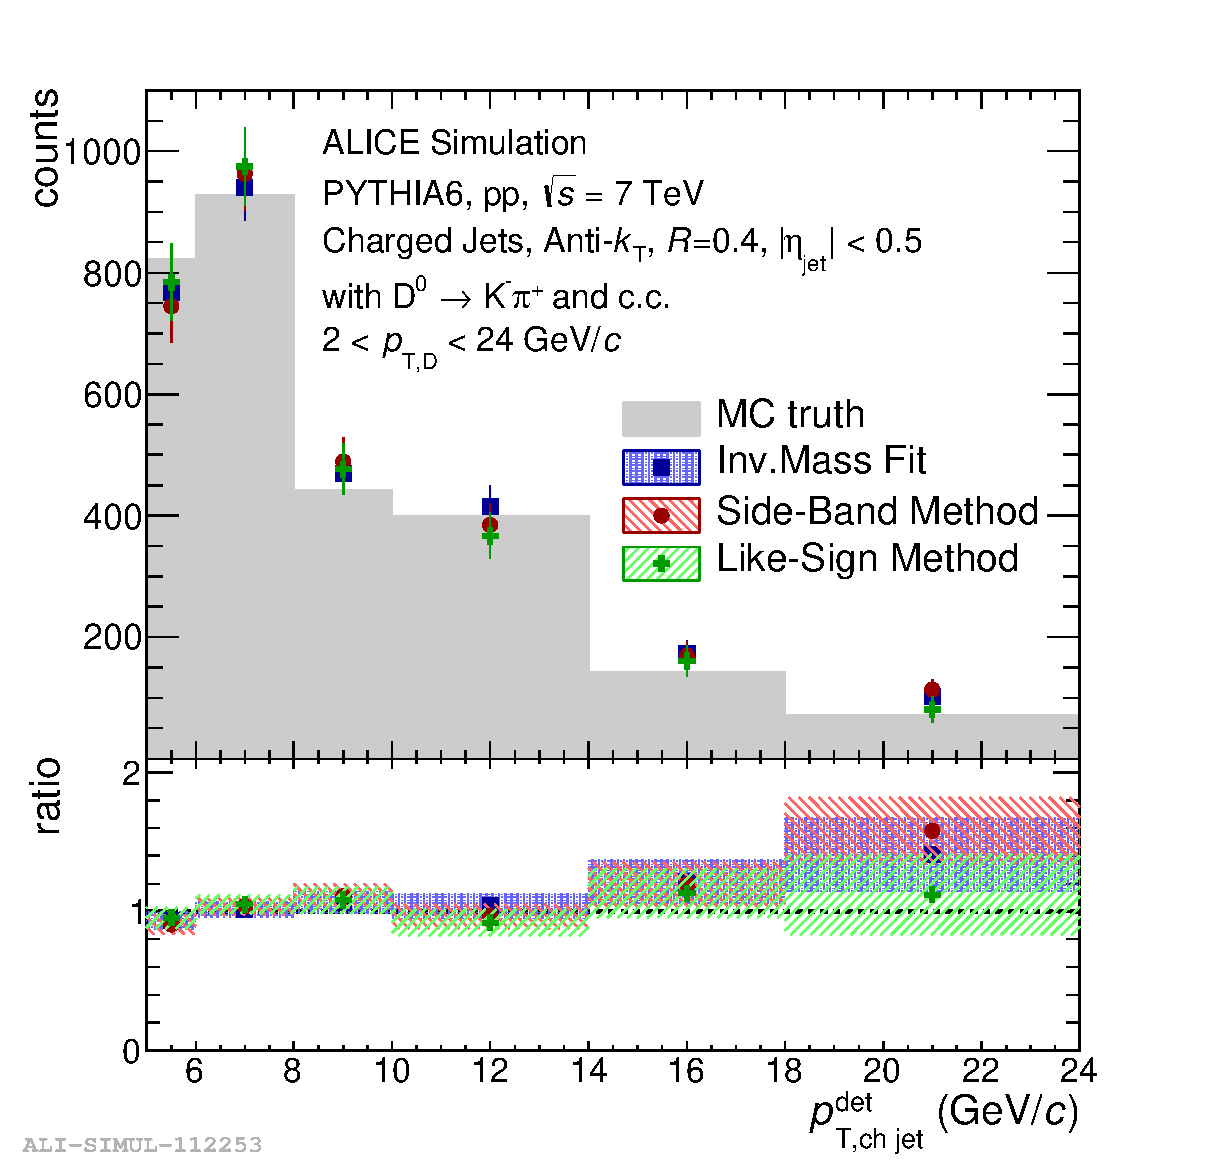
\includegraphics[width=.57\textwidth]{img/HQ16_Simulation_MethodComparison}\hspace{1pc}%
\begin{minipage}[b]{.39\textwidth}\caption{\label{label}Figure caption for a narrow figure where the caption is put at the side of the figure.}
\end{minipage}
\end{figure}

\section{Conclusions}


\section*{References}
\bibliography{biblio}{}
\bibliographystyle{iopart-num}

\end{document}


